\documentclass[9pt,twocolumn,twoside]{fernandes_paper} 
%Default opts:9pt,twocolumn,twoside
\graphicspath{{images_paper/}}

\newcommand{\KB}[1]{\noindent\color{blue}$\Longrightarrow$ #1\normalcolor}
% \newcommand{\mf}[1]{\noindent\color{color2}\sethlcolor{cyan}\hl{$\Longrightarrow$#1}\normalcolor}
\newcommand{\mf}[1]{\noindent\color{orange}{$\Longrightarrow$#1}\normalcolor}


\title{Design Principles from Glass Sponges \\for Structurally Robust Lattices}

\author[1]{Matheus C. Fernandes}
\author[2]{James C. Weaver}
\author[1,2,3]{Joanna Aizenberg}
\author[1,2,3,*]{Katia Bertoldi}

\affil[1]{John A. Paulson School of Engineering and Applied Sciences -- Harvard University, Cambridge, MA 02138}
\affil[2]{Wyss Institute -- Harvard University, Cambridge, MA 02138}
\affil[3]{Kavli Institute -- Harvard University, Cambridge, MA 02138}
\affil[*]{Corresponding author: \href{mailto:bertoldi@seas.harvard.edu}{bertoldi@seas.harvard.edu}}

\keywords{Architected materials, truss structure, square lattice, buckling resistance, glass sponges, bio-inspired engineering.}

\begin{document}
\maketitle
% \doublespace
\linenumbers

\begin{figure*}[!htb]
    \centering
    \captionsetup{width=0.8\textwidth}
    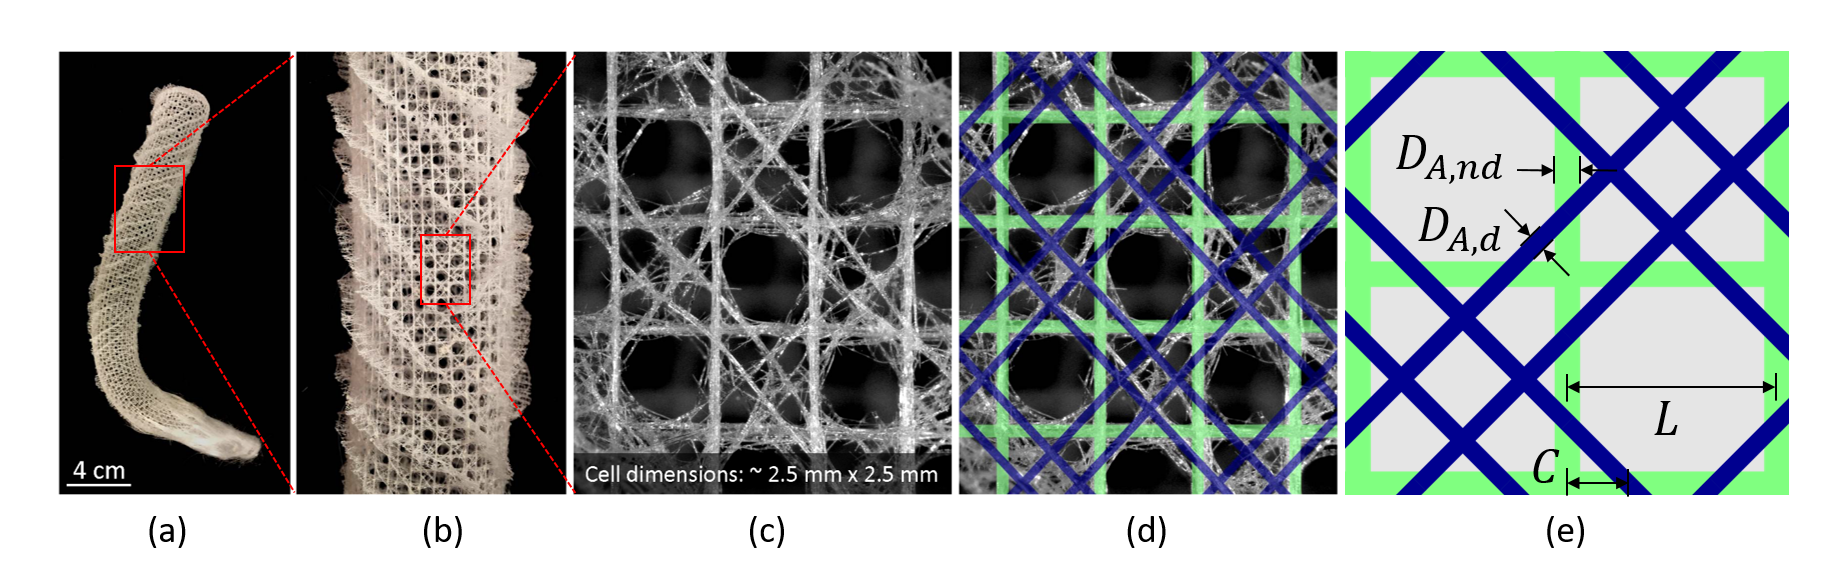
\includegraphics[width=0.6\textwidth]{Fig1}
    \caption{\textbf{Hexactinellid sponge \textit{Euplectella aspergillum.}} (a)-(b) Full-frame photo of sponge. (c) Close up microscope image of the sponge. (d) Comparison between the idealized model (green and blue lines) and the sponge structure.}\label{Fig1}
\end{figure*}

\begin{figure*}[!htb]
	\centering
	\captionsetup{width=0.8\textwidth}
	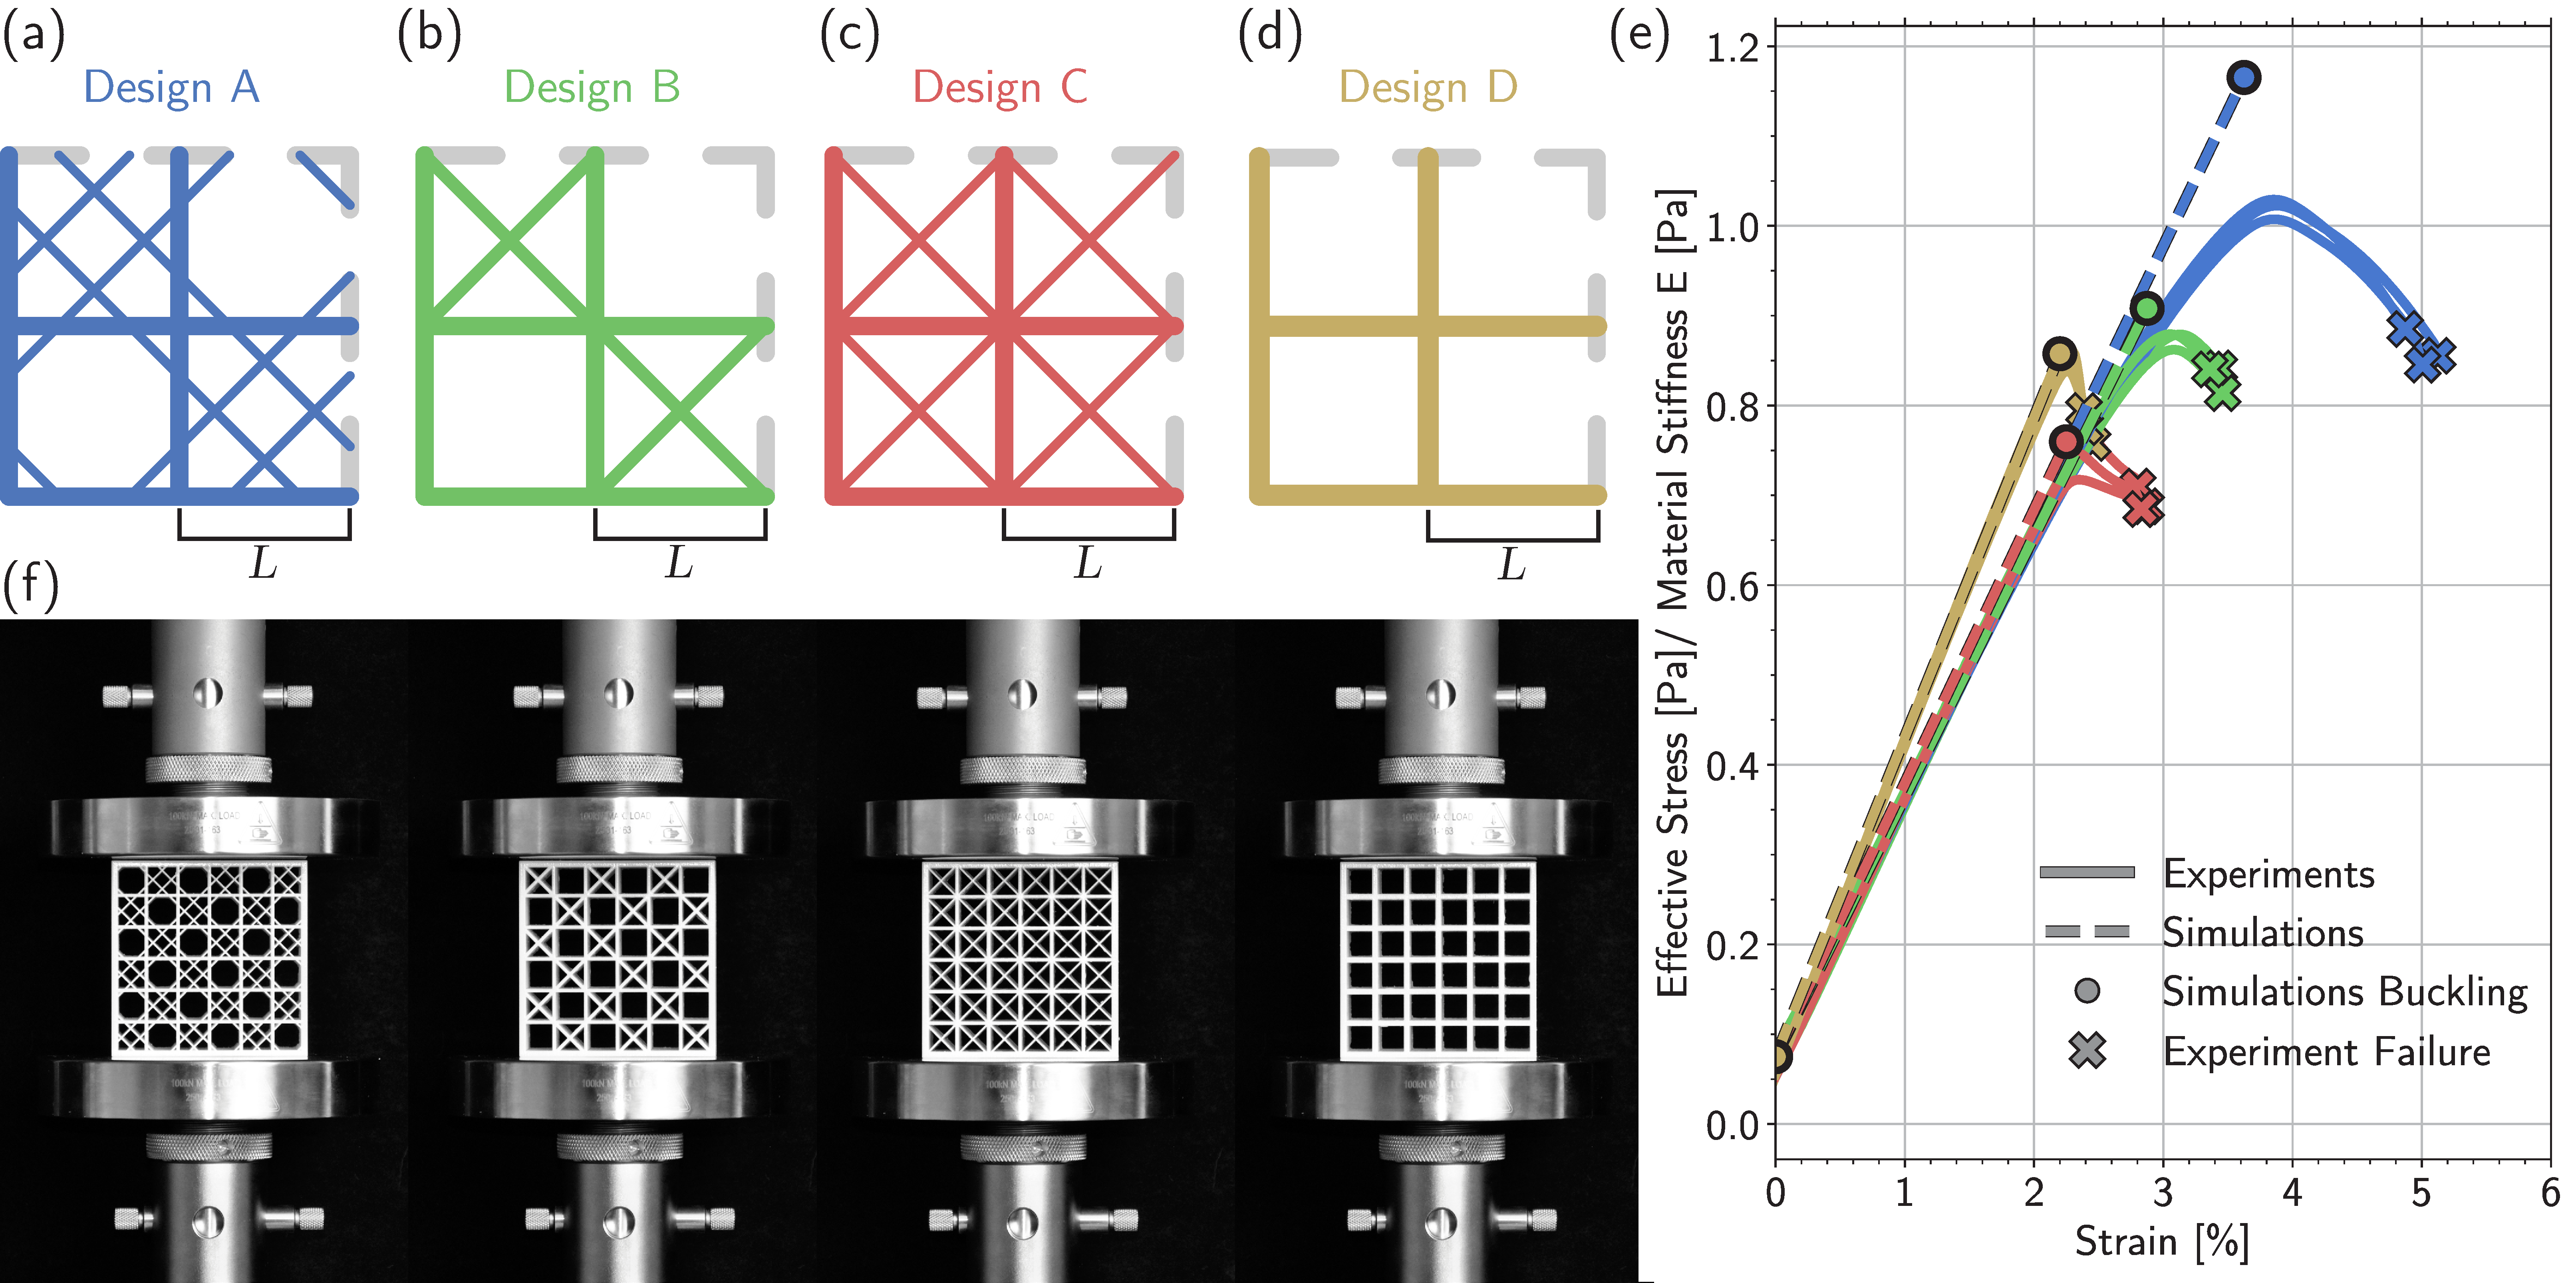
\includegraphics[width=0.9\textwidth]{Fig2}
	\caption{\textbf{Experimental Results.} (a)-(d) shows the different designs (\emph{Design A-D}) considered in this analysis. (e) shows the undeformed experimental setup for the different designs. (f) shows the experimental stress-strain curve as well as the overlaid numerical results for linear stiffness and critical buckling for the different designs considered.}\label{Fig2}
\end{figure*}

The hexactinellida sponge \textit{Euplectella Asperguillum} species, commonly known as the Venus' Flower Basket, has received significant attention in the engineering and material science communities for its remarkable hierarchical design and robustness across many scales. Its fundamental building blocks, called spicules, are constructed using laminated skeletal elements which consist of a central protein-based organic core surrounded by alternating concentric domains of consolidated silica nanoparticles (clear glass) and organic interlayers. \cite{weaver2010,aizenberg2005,shulze1887} Remarkably, these spicules are arranged to form a regular and complex square-grid architecture reinforced by a set of double diagonals (a set of two diagonals going in each direction), creating a checkerboard-like pattern of alternating open-closed cells (see \cref{Fig1}). Notably, while it has been demonstrated that the laminar architecture of the spicule leads to superior resistance to fracture propagation \cite{miserez2008} and the shape of the spicules enhances the overall strength against buckling \cite{monn2015}, the functionality of the complex double diagonal square-grid macroscale structure is still unknown. 

The macro-scale architecture of the \textit{Euplectella Asperguillum} provides a remarkable example of slender and regular lattice-like material constructed by nature. Such lattice materials have recently demonstrated to offer novel and unique properties, including being light weight, \cite{schaedler2011,ashby2006} having high energy absorption, \cite{evans2001} and having the ability to control the propagation of waves \cite{phani2006} as well as heat flow. \cite{lu1998,ashby1997,evans1998} Generally speaking, the properties and functionality of such materials are  dictated by the node connectivity. In particular, a minimum node connectivity of 6 is required for 2D lattice materials to be  stretching-dominated, and therefore,  more weight-efficient for structural applications. \cite{deshpande2001} As such, lattice materials with square architecture (which has a node connectivity of 4) are known to be very unstable when loaded along specific directions (as the only shear resistance arises from the joints) \cite{gibson1999} and typically require diagonal bracings to stabilize them.\cite{phani2017}

In this paper, we use the anatomy of the hexactinellid sponge species \textit{Euplectella Aspergilum} skeletal system as inspiration for the design of mechanically robust lattice materials with square architecture. First, we use a combination of experiments and numerical analyses to understand the overarching mechanical functions driving the particular and regular alignment of trusses found in the sponge. Then, we utilize an optimization algorithm based on the principles introduced by the sponge to determine the  configuration of reinforced square lattice that achieve the highest mechanical performance. Therefore, our results indicate that the  principles used by Nature to design the \textit{Euplectella Aspergilum}  may guide the design of lattice architectures structurally more robust than those currently used in modern devices and infrastructure.

To understand the role of the sponge architecture, we start by comparing its performance to that of additional three 2D lattices, all based on a square architecture with edge lengths $L$ (see Supplementary Materials for details). Specifically,  we  consider:
\emph{Design A}  which is inspired by the sponge and comprises a set of double diagonals going in opposite directions (see \cref{Fig2}(a)); \emph{Design B}  which is similar to the sponge design but only contains a single diagonal crossing each of the closed cells (see \cref{Fig2}(b)); \emph{Design C} which is similar to bracings found in modern structural engineering and contains a crossing set of diagonal beams in every cell (see \cref{Fig2}(c)); and \emph{Design D}  which  has no diagonal reinforcement (see \cref{Fig2}(d)). In all our designs we consider struts with rectangular cross section and depth large enough to avoid any out-of-plane deformation. Moreover, to ensure a fair mechanical comparison between the four designs, we keep the total mass constant and
for \emph{Designs A, B}, and \emph{C} we also constrain the  ratio between the mass of the diagonals and non-diagonals struts to be identical (see Supplementary Materials for details).  %Finally, in all our analyses we constraint the lattices to deform in-plane. To this end, in our experiments we consider specimens sufficiently thick for which out-of-plane deformation is negligible and in the the numerical simulations we assume plane-strain conditions.  

We began our analysis by testing samples of the four considered designs comprising a tessellation of $6\times6$ square cells with $L=1.91$ cm. The samples were fabricated with a multi-material 3D printer \mf{(add model @James)} using \KB{name of material @James} and compressed uniaxially using an Instron Model 5969 with 50kN capacity (\Cref{Fig2}(e)). For each design, we 3D print three separate specimens that are then reported in \cref{Fig2}(f). The results reported in \Cref{Fig2}(f) show that all structures are characterized by an initial linear behavior, a sudden departure from linearity caused by in-plane buckling and catastrophic failure following immediately thereafter. Furthermore, it is also important to note that all designs with diagonal reinforcement (i.e. \emph{Designs A-C}) overlay each other in the linear regime. Focusing on the initial linear regime, we find that  the different diagonal reinforcement designs considered do not impact the structure's overall stiffness (i.e. the initial stiffness of Designs A, B and C are identical). Design D, as expected, has a higher stiffness because of its thicker vertical and horizontal elements. However, it fails much earlier due to a shorter critical buckling strain. On the other hand, \emph{Design A} (the sponge design) outperforms the considered structures in the amount of load it can bare before the onset of buckling occurs and provides the best mechanical performance without compromising the structural stiffness while using the same total amount of material.

Next, we use Finite Element (FE) simulations conducted with the widely used commercial software ABAQUS/Standard to further understand how the double diagonal system found in the \textit{Euplectella Aspergilum} results in significantly improved mechanical performance. All our models are constructed using Timoshenko beam elements (ABAQUS element type B22) and the material's response is captured using an isotropic linear elastic materials. We start by simulating the response of the 6 by 6 specimens tested in our experiments and find very good agreement between our experiments and numerical model (see \cref{Fig2}(f)). Having validated our numerical analysis with experimental results, we next use the numerical model to investigate the first-order behavior of the structure (neglecting all edge effects by the assumption of an infinite periodic structure). To reduce the computational cost, we took advantage of the periodicity of the structures and investigated their response by considering a Representative Volume Element (RVE) with periodic boundary conditions along the free edges of the unit cell (more information on this can be found in the SI). In an effort to create a method for impartial comparison, we maintain a constant total mass (or constant volume as the material is assumed to be incompressible) between all of the designs, as well as a constant mass ratio between diagonal and non-diagonal elements for the designs containing diagonal reinforcement. 

The results presented in \cref{Fig3}(a) show that all of the structures containing diagonal reinforcement behave the same way for varying loading angles. This illustrates the fact that the structural stiffness is independent of design, but instead depend on the amount of material allocated to elements aligned parallel to the angle of loading. This is further supported by the graph for \emph{Design D}, where all of the material from the diagonal beams is removed and allocated to the non-diagonal elements, giving the structure a higher stiffness at $0^\circ$ and lower stiffness at $45^\circ$. Any stiffness at $45^\circ$ in Design D is strictly a result of the bending resistance due to the pinned joints between the non-diagonal beams.

The results shown in \cref{Fig3}(b) indicate that the structural buckling strength is clearly dependent on the design and alignment of the beam elements. From this figure, we can see that \emph{Design A}, the sponge design, has the highest buckling strength compared to the other designs containing diagonal reinforcement. At $45^\circ$ loading, Design A improves the buckling strength by a factor of 2.5 times that of \emph{Design C}, which is the commonly used truss systems. 

Multiplying the results of \cref{Fig3}(a) together with \cref{Fig3}(b) provides a measure of the normalized critical buckling load as seen in \cref{Fig3}(c). From these results, we clearly see that the geometric benefit attributed to \emph{Design A} clearly propagates through all loading angles. The benefit presented, is substantial near $0^\circ$ loading angles from all other designs. For loading angles near $\approx 45 ^\circ$, \emph{Design A} still outperforms \emph{Design B} and \emph{Design C}. However, it is important to note that \emph{Design D} appears to have a benefit over \emph{Design A} in this regime. This benefit, however, is attributed to numerical constraints imposed by the periodic boundary conditions. When creating a finite size structure and omit and peridic boundary conditions from our model, we see the benefit of \emph{Design D} over \emph{Design A} vanish and \emph{Design A} outperforms over all other considered designs for all loading angles. This further benefit for \emph{Design A} is attributed to it's insensitivity to edge effects. Furthermore, from \cref{Fig3}(e), we can see that \emph{Design A}, \emph{Design B}, \emph{Design C} have periodic buckling modes that are note dependent on the domain size, whereas for \emph{Design D}, the buckling mode strongly depends on the domain size (find further analysis on varying loading angles in the SI.)

\mf{write section on Optimization here}

In summary, the investigation of the \textit{Euplectella Asperguillum's} intricate and regular structure has lead to macro-scale design principles that can be applied to general square lattice materials and structures. When compared with other diagonally reinforced square lattice designs, the sponge design has experimentally and numerically proven to provide a superior mechanism for withstanding loads prior to onset of buckling. By controlling the number of diagonals, diagonal separation and mass ratio between diagonal and non-diagonal elements, a structure's design can be optimized to withstand buckling load caring capacity. 

\section*{Acknowledgments}
 \noindent This work was partially supported by: NSF-GRFP Fellowship  Grant\# DGE-1144152 (for M. C. F.), GEM Consortium Fellowship (for M. C. F.), the Harvard Graduate Prize Fellowship (for M. C. F.), \mf{add whatever else here}.
 We would also like to thank James R. Rice, Mark Scott, Joost Vlassak, and Chris Rycroft for insightful discussions.

\begin{figure*}[!htb]
	\centering
	\captionsetup{width=0.8\textwidth}
	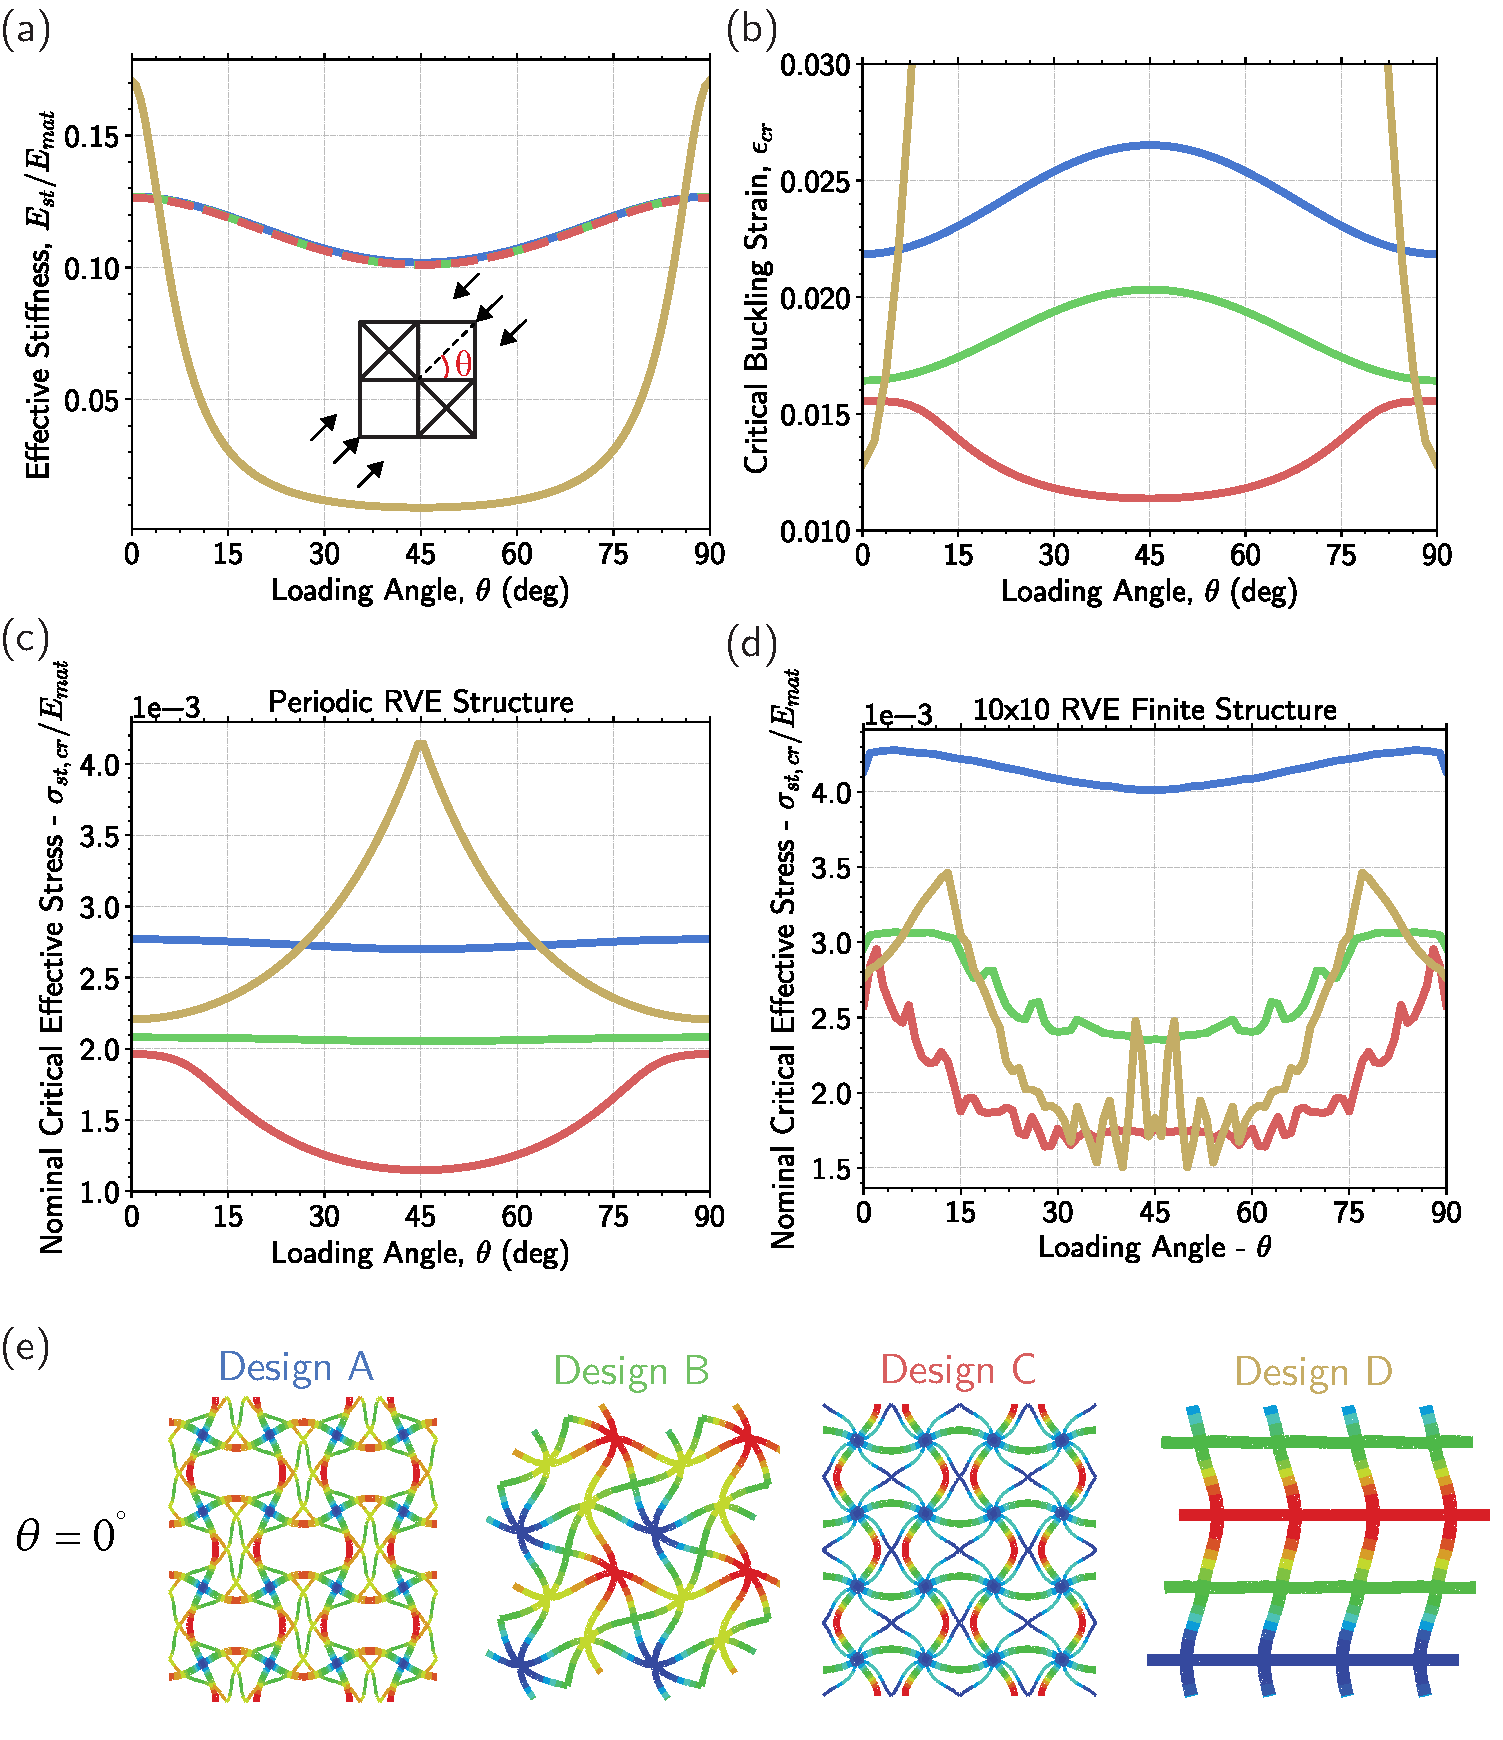
\includegraphics[width=0.7\textwidth]{Fig3}
	\caption{\textbf{Structure Mechanical Response} Figure showing (a) the structural stiffness for the different designs and (b) the buckling resistance for the different designs. The designs considered are depicted below as \emph{Design A-D.}} \label{Fig3}
\end{figure*}

\begin{figure*}[!htb]
	\centering
	\captionsetup{width=0.8\textwidth}
	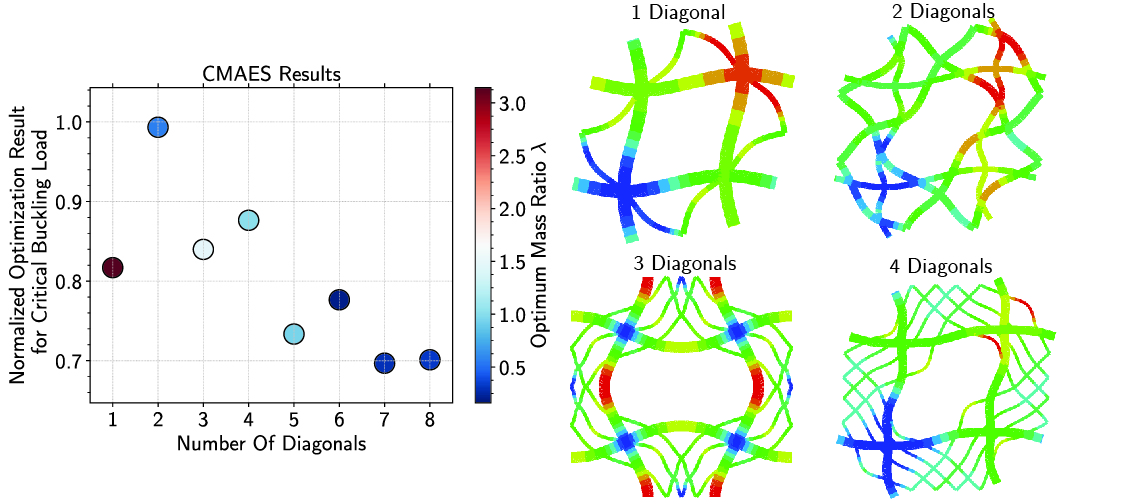
\includegraphics[width=0.7\textwidth]{Fig4}
	\caption{\textbf{Critical Buckling Load Optimization Results.} (a) shows the optimal value of critical buckling load for varying number of diagonals. The color of each point represents the optimal mass ratio $\lambda$  parameter for that configuration.  Note, we do not explicitly show the other optimal values for the diagonal spacing parameters. (b) shows the resulting deformed geometries for designs including one to four diagonals.} \label{Fig4}
\end{figure*}

\noindent\rule[-1.5ex]{\linewidth}{1pt}
%\nocite{*}
\bibliography{refs}
%\bibliographystyle{apalike}
%\bibliographystyle{plainnat}
\bibliographystyle{unsrtnat}


\end{document}